\documentclass[12pt]{article}

\usepackage{amsmath}
\usepackage{amsfonts}
\usepackage{hyperref}
\usepackage{enumitem}
\usepackage{graphicx}
\usepackage{abstract}
\usepackage{geometry}

% page settings
\geometry{a4paper, margin=1in} % sets A4 paper with 1-inch margins

% Title Page
\title{\textbf{Discrete Bulk Reconstruction Problem} \\ \large Compiled Research}
\author{Piper Jeffries \\ Missouri S\&T \\ \texttt{pejbvy@umsystem.edu}}
\date{\today}

\begin{document}

\maketitle

%%%%%%%%%%%%%%% ABSTRACT %%%%%%%%%%%%%%%%%%%%%%%%%%%%%%
\begin{abstract}
    The \textbf{Discrete Bulk Reconstruction Problem (DBRP)} models the entanglement structure of quantum systems using discrete graphs. It is rooted in the Anti-de Sitter / Conformal Field Theory (AdS/CFT) correspondence, which connects a gravitational theory in AdS space (the bulk) to its quantum field theory on its boundary (the CFT).
    While this describes a universe different from our own, it offers valuable insights into quantum gravity and spacetime emergence. 
    \\
    \indent Instead of using traditional approaches that rely on continous AdS space, DBRP models the bulk as a graph, where nodes correspond to regions of space and edge weights encode entanglement connectivity.
    In this framework, geodesics in AdS are approximated by min-cuts in the graph, and the Ryu-Takayanagi (RT) formula determines minimal surfaces in the bulk, allowing for bulk geometry reconstruction from boundary entanglement.
    \\
   \indent DBRP leverages tensory networks and holography to provide a discrete approach to understanding spacetime, quantum entanglement, and information flow.
    DBRP could provide profound insight in quantum gravity, improved quantum error correction, and practical quantum computing applications.
\end{abstract}

\newpage 
\tableofcontents
\newpage

%%%%%%%%%%%%%% INTRO %%%%%%%%%%%%%%%%%%%%%%%%%%
\section{Introduction}
    \hspace{0.5cm} DBRP aims to reconstruct spacetime (the bulk) from the entanglement structure of quantum systems. This structure is defined by the collection of entanglement entropies of its subsystems, which quantify how much information a given region of the system contains. More precisely, entanglement entropy measures how strongly a subsystem is correlated with the rest of the system.
    \\
    \indent A key motivation for DBRP comes from the AdS/CFT correspondence, first proposed by Juan Maldacena in 1997. This duality suggests that a (d + 1)-dimensional anti-de Sitter (AdS) space, which includes quantum gravity, is fully encoded by a d-dimensional conformal field theory (CFT) on its boundary. Because the CFT is non-gravitational, computations are easier, making this framework a powerful tool for understanding quantum gravity.
    \\
    \indent By leveraging insights from AdS/CFT, DBRP offers a discrete, graph-based approach to bulk reconstruction, which allows for a new perspective on how spacetime emerges from entanglement, with potential applications in both holography and quantum information theory.

%%%%%%%%%%%%%%%% 2 %%%%%%%%%%%%%%%%%%%%%%%%%%%%
%%%%%%%%%%%%%% All about AdS/ CFT space %%%%%%%%%%%%%%%%%%%%%%%%
    \subsection{AdS (Anti-de Sitter) Space $\Rightarrow$ The Bulk}
        \begin{itemize}
            \item The \textbf{bulk} represents a higher-dimensional space in the AdS/CFT framework.  
            \item A \textbf{surface} is a geometric object within AdS space that plays a crucial role in holography.  
            \item The \textbf{minimal area} surface, also known as the RT surface in AdS/CFT, spans the boundary subregion and has the smallest possible area.  
            \item Since direct calculations in the bulk are challenging due to quantum gravity, computations are instead performed on the CFT boundary.  
        \end{itemize}

    \subsection{CFT (Conformal Field Theory) Space $\Rightarrow$ The Boundary}
        \begin{itemize}
            \item The \textbf{boundary} represents a lower-dimensional space that forms the "edge" or "boundary" of the AdS bulk.
            \item The \textbf{CFT} is a non-gravitational theory that lives on the boundary of the AdS spacetime.
            \item The information of the boundary is encoded in the bulk. The bulk and boundary are related by the holographic principle.
        \end{itemize}

        %% Photo of AdS/ CFT space 
        \begin{figure}[htbp]
            \centering
            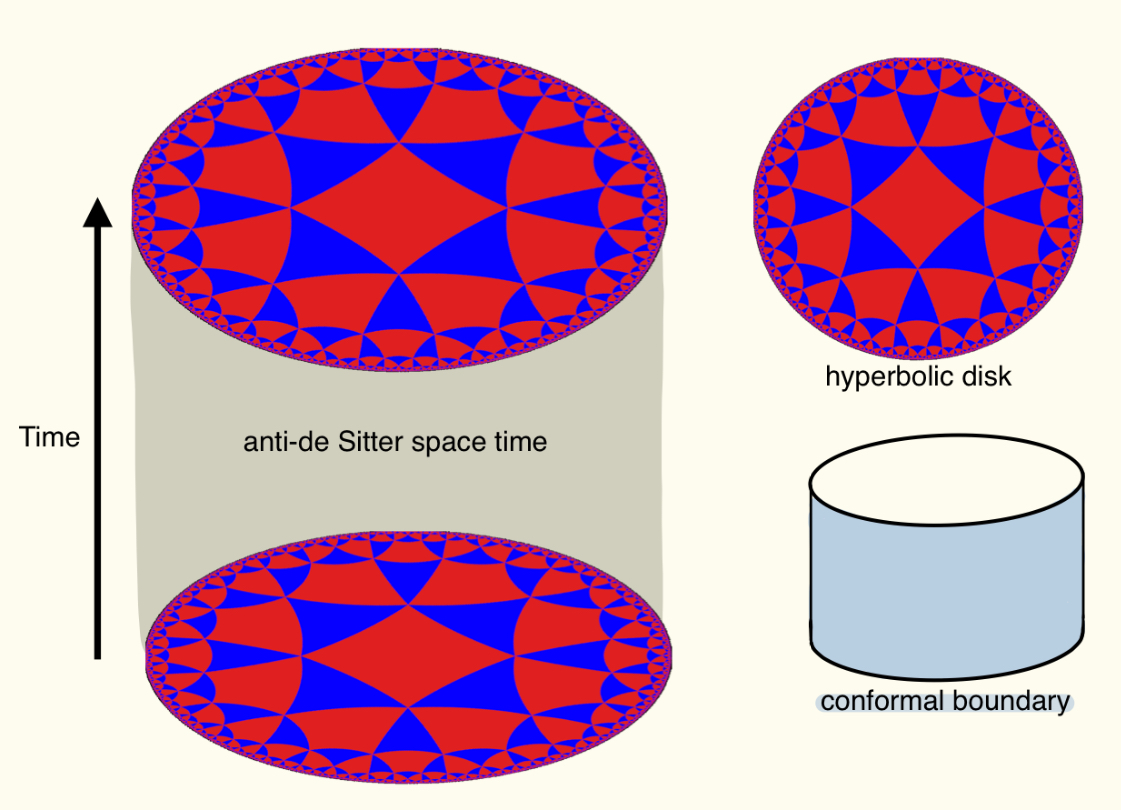
\includegraphics[width=0.8\textwidth]{ads_cft.jpeg}  
            \caption{This illustration shows the AdS/CFT spacetime, where the AdS can be thought of as soup in the can and CFT is the soup can label. A geodesic is a straight line across the hyperbolic disk, which is the shortest path between points. In the context of anti-de Sitter spacetime, a geodesic represents the path that a particle follows when only affected by gravity.}  
            \label{fig:AdS/CFT space}  
        \end{figure}

        \newpage
        When dealing with a 5-dimensional AdS bulk, the boundary is typically 4-dimensional, and the CFT lives on this 4-dimensional boundary. This illustrates the idea that the boundary is one dimension less than the bulk. The boundary is where we will perform our computations, as it is easier to compute without gravity. Using the CFT, we can reconstruct the gravitational dynamics of the AdS bulk, which corresponds to the geodesics of the hyperbolic disk. Geodesics in AdS space are curved, unlike straight lines in flat geometry, even though they represent the shortest path between points. This curvature reflects the negative curvature of AdS space and the effects of gravity.

        These gravitational dynamics come from the entanglement entropy in the CFT. In AdS/CFT, the entanglement entropy on the boundary CFT encodes information about the geometry of the bulk. Given a CFT state, we can determine the corresponding spacetime that the CFT describes, including its geometry and gravitational dynamics. This allows us to extract bulk information, such as spacetime curvature, directly from the boundary CFT state. Thus, we can use the CFT to reconstruct the AdS bulk.

        \textbf{AdS/CFT correspondence} means that the gravitational theory in the bulk is equivalent to the non-gravitational CFT on the boundary. In other words, the two theories describe the same physics but from different perspectives: one is a gravitational theory, and the other is a quantum field theory without gravity. This is an extraordinary idea because it suggests that gravity can be understood in terms of a simpler quantum field theory on the boundary, offering insights into quantum gravity through non-gravitational methods.

    \subsection{Holographic Principle}
        The \textbf{Holographic Principle} is central to the AdS/CFT correspondence. It states that a lower-dimensional, non-gravitational theory (CFT) can fully describe the physics of a higher-dimensional gravitational theory (AdS). More formally, this principle suggests that the physics within a region of space can be described by a theory defined on the boundary of that region, without the need to describe the bulk independently.

        This discovery is important because it suggests that quantum gravity, which typically involves understanding the behavior of spacetime and gravity in the bulk, can be described by a simpler theory on the boundary. In this context, we don't need to deal directly with quantum gravity in the bulk; instead, we can use quantum field theory on the boundary, which does not involve gravity. This provides a new framework for studying gravitational phenomena without directly engaging with the complexities of quantum gravity. 

        \textbf{Holographic Relationship} means that everything happening in the bulk AdS spacetime can be described by the boundary CFT, and vice versa. The idea is that the bulk gravitational dynamics are encoded in the CFT through entanglement and other quantum information properties, while the CFT state encapsulates all the physics of the bulk region.

        The holographic relationship consists of two theories:
        \begin{itemize}
            \item A theory of quantum gravity (the AdS bulk) and a quantum field theory without gravity (the CFT boundary). The relationship between the two theories is called "holographic," which is where the term "holographic relationship" comes from.
            \item \textbf{Note:} The equivalence of these theories is still a subject of ongoing research and has not yet been fully proven in all generalities. The mapping between the two theories has yet to be completely developed, and much of the work involves finding more specific correspondences between the two.
        \end{itemize}

        A holographic relationship means there exists a mapping or "dictionary" that maps all states and observables from one theory to a corresponding state and observable in the other. For example, bulk field configurations map to boundary operators, and bulk entanglement corresponds to boundary entanglement entropy. Currently, we lack a full dictionary for the AdS side, and researchers are actively working to establish more complete mappings and further validate the holographic principle.

    \subsection{Spacetime Geometry and What It Means in AdS/CFT Space}
        \hspace{0.5cm} Gravity is the curvature of spacetime caused by mass and energy. The "geometry" of spacetime refers to this curvature. If there is no gravity, the geometry is simple and uncurved.

        In AdS space, geometry is negatively curved due to the nature of its spacetime structure. This leads to a spacetime geometry that is "hyperbolic," meaning it has negative curvature at every point. The CFT can reconstruct the geometry of the AdS bulk, meaning that data from the CFT can be used to determine the shape or curvature of spacetime in the AdS bulk.

        \textbf{Entanglement is directly related to the geometry of the bulk spacetime:}
        \begin{enumerate}
            \item The amount of entanglement in different regions of the CFT tells us about the structure and curvature of the corresponding bulk spacetime in AdS.
            \item More entanglement on the boundary implies more curvature or structure in the bulk geometry.
            \item Proven with the RT formula: more entanglement = larger minimal surface area = more curved and intricate bulk geometry.
        \end{enumerate}

    \subsection{Why Is This Important?}
        \hspace{0.5cm} The shape of spacetime tells us how gravity behaves. If we can reconstruct the bulk geometry from the CFT, we can gain insights into the quantum aspects of gravity and understand how measurements (or experiments) on the boundary affect the information encoded in the bulk. This could lead to a deeper understanding of quantum gravity and its connection to quantum field theory.

%%%%%%%%%%%%%%%%%%% 3 %%%%%%%%%%%%%%%%%%%%%%%%%%%%%%%%%
%%%%%%%%%%%%%%%% RT formula %%%%%%%%%%%%%%%%%%%%%%%%%%%%%%%%%%%%
\section{Ryu-Takayanagi}
        \hspace{.5cm} It is important to note that there is no need to calculate the entanglement between subsystems. DBRP initially states full AdS/CFT correspondence.

    \subsection{Von Neumann entropy}
        Formal definition:
        \[
            S(\rho_A) = -Tr(\rho_{A}log\rho_A)
        \]
        \hspace{0.5cm} In DBRP, we do not compute $S(\rho_A)$ directly; instead, the entropy values are provided as inputs and implicitly follow this definition. Von Neumann entropy measures the uncertainty or entanglement of a subsystem.
        \begin{itemize}
            \item If $\rho_A$ is a pure state ($S=0$), subsystem A is not entangled with the rest.
            \item If $\rho_A$ is highly mixed (large $S$), then A is strongly entangled with the rest of the system.
        \end{itemize}

        In the holographic context, Von Neumann entropy describes entanglement entropy in the boundary CFT. However, in DBRP, these entropy values are not computed from wavefunctions but are instead given as problem constraints to reconstruct the bulk geometry via min-cut methods.
    
    \subsection{Minimal area of bulk surface}
        \hspace{0.5cm} In the higher-dimensional bulk space (AdS), there exists a surface whose area corresponds to the entanglement entropy of a boundary region. The smallest possible area of this surface, known as the RT surface, is proportional to the entropy of the boundary subregion. The more entangled a boundary region is, the larger the area of its corresponding minimal surface in the AdS bulk.        

    \subsection{Ryu-Takayanagi (RT Formula)}
        \hspace{0.5cm} RT forumla calculates the minimal entanglement entropy in a holographic system by identifying the smallest possible surace that seperates a boundary region from the rest of the system. RT formula states entangelment entropy of subregion A is:
        \[
            S(A) = \frac{Area(\gamma_A)}{4G_N}
        \]
        \hspace{0.5cm}Where $\gamma_A$ is the minimal surface in the bulk that seperates A from the rest of the system and $G_N$ is Newton's gravitational constant.
        \\
        \vspace{0.3cm}

        \hspace{0.5cm} \textit{Ryu-Takayanagi} is a key entry in the holographic dictionary. Where the holographic dictionary refers to the correspondence between the AdS/CFT space. This dictionary relates quantum entanglement in the boundary CFT to geometric structures in the AdS bulk. In particular, the RT formula expresses entanglement entropy as the area of a minimal surface in the bulk. DBRP leverages this principle by using min-cut methods to reconstruct the bulk graphs from entanglement entropy data. Which allows us to implement a discrete version of this holographic mapping.
        \\

        \hspace{0.5cm} If you know what the minimal area of a subsystem is, you know the entanglement entropy of said subsystem with the rest of the system. Therefore, you know the amount of quantum information in subsystem.

%%%%%%%%%%%%%%%%% DBRP %%%%%%%%%%%%%%%%%%%%%%%%%%%%%%%%%%%%%%%%%%%%%%
\section{Discrete Bulk Reconstruction Problem}
\subsection{Background Information}
    \hspace{0.5cm}A \textbf{Hilbert space} is a mathematical framework used to describe quantum states. Quantum states exist as vecots in a Hilbert space, where they follow the principles of superposition and inner product structures.
    \\
    For example, a single qubit lives in a two-dimensional Hilbert space. More generally, for n-qubit system, the corresponding Hilbert space has dimension $2^n$, meaning the number of possible quantum states grows exponentially with the number of qubits.
    
    \vspace{0.3cm}

    \indent A \textbf{Tensor Product} is a mathematical operation used to describe composite quantum systems. If we have two subsystems, their total Hilbert space is the \textbf{tensor product} of their individual Hilbert spaces: 
    \[
        \mathcal{H}_{AB} = \mathcal{H}_{A} \otimes \mathcal{H}_B
    \]
    This operation combines two or more Hilbert spaces into a single composite space, allowing for entanglment between subsystems. 

\subsection{Min-Cut Theory}
Formal Definition:
\\
Given a finite weighted undirected graph \( G \) with real edge weights \( w(e) \geq 0 \), as well as two disjoint vertices \( R, R' \), a min-cut is a set \( C \) of edges with minimum total weight
    \[
    W = \sum_{e \in C} w(e)
    \]
whose removal disconnects \( R \) from \( R' \).

In the AdS/CFT correspondence, entanglement entropy in the boundary CFT is geometrically represented by minimal surfaces in the bulk (via the Ryu-Takayanagi (RT) formula). In DBRP, we replace the continuous bulk geometry with a discrete graph, where entanglement entropy values are mapped to edge weights.

The min-cut of this graph corresponds to minimal bulk surfaces, allowing entropy calculations without requiring a continuous bulk metric. By applying min-cut theory, DBRP reconstructs the bulk while ensuring a structure that is consistent with quantum error correction properties in holography.

Min-cut is used as a verification tool to ensure that the graph created properly represents the quantum information properties of the system.
We use it to verify the graph properly reproduces individual entropy values, strong subadditivity, and monogamy of mutual information.

\subsection{Problem Initalization}
Start with creating combined Hilbert space for each N atomic boundary subregions:
\[
\mathcal{H} = \otimes^{N}_{i=1}\mathcal{H}_{i}
\]

The bulk can be modeled by a weighted undirected graph where each subregion is an RT (or minimal area) surface, which corresponds to min-cuts in \( G \).

\begin{figure}[htbp]  % 'h' places the figure "here" (can be adjusted)
    \centering
    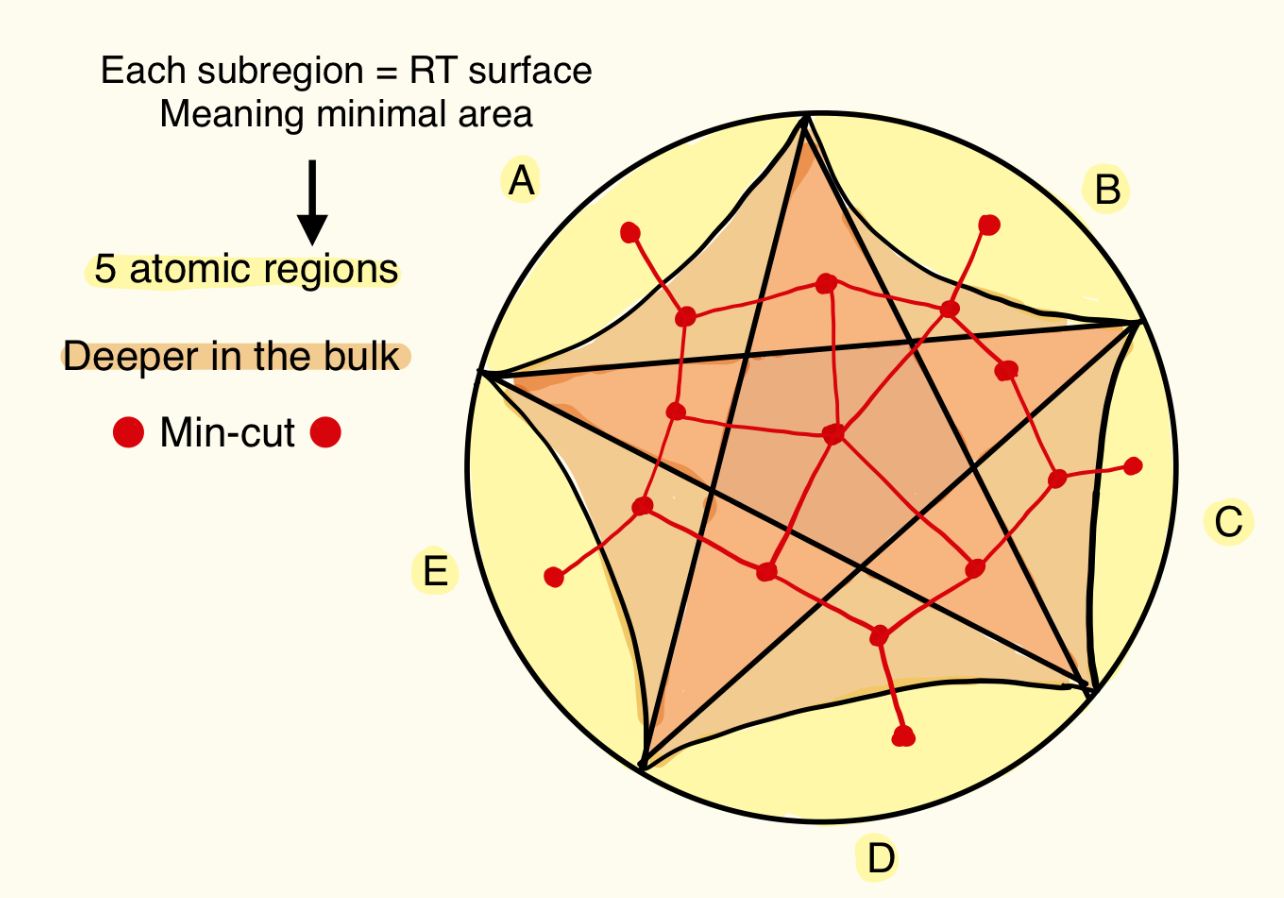
\includegraphics[width=0.6\textwidth, height=0.23\textheight]{mincut_graph.jpeg}  % Adjust width as needed
    \caption{5 atomic region weighted undirected graph model of the bulk. Where each subregion is cutting deeper into the bulk. Each subregion is a minimal surface (RT surface) and is connected by the min-cut (red) line.}  % Caption text
    \label{fig:mincut}  % Label for referencing
\end{figure}

\subsection{Official Problem Statement}
\hspace{0.5cm} Given as input a list of atomic boundary regions labeled \( 1, \dots, N \), a list of subsets of the regions \( R_1, \dots, R_k \subseteq [N] \), and a real-valued entropy \( S(R_i) \geq 0 \) for each \( R_i \), the weight of the minimum cut separating \( R_i \) from the rest of the boundary vertices (i.e., from \( [N] - R_i \)) is equal to \( S(R_i) \).


\subsection{General Idea}
\hspace{0.5cm} If we are given a complete entanglement structure of the boundary we can reconstruct the bulk graph using the min-cut principle. Given a set of entropy values for different boundary subsystems and lines (edges) representing connectivity, the goal is to place entropy values in a way that minimum cuts across edges math the entanglement structure of the system. Min-cut correspond to entanglement entropy, therefore adjust where the values go to satisfy this relationship.
\\
\indent After applying min-cut and entropy values are assigned correctly, bulk geometry emerges as a discrete graph. Which provides insight into how spacetime itself emerges from entanglement structure in holography. 

\textbf{This is basically the inverse min-cut problem.} Now we are given min-cut, find graph that gave you min-cut solution, therefore this graph is not unique. While the graph is not unique you can add on additional properties. For example, planar, few vertices. For this problem assume no wormholes. For DBRP to work we need to ensure all quantum states satisfies properties (more on that later). \\
\\
\indent In order for DBRP to work we have to prove it is computable. Computable means it has an upper bound.
Therefore, we will prove DBRP has an upper bound of $2^{2^N}$.

\subsection{Upper Bound Proof}
Given $K\leq2^N$ boundary regions form all $\leq2^N$ possible intersections of RT regions. At most 1 vertex needed in each region. Using linear programs to determine edge weight takes "only" exp(exp(exp(N))) time!

\subsection{Determining Edge Weights}
Use linear programming, for every possibility of what min-cuts could be try to solve some linear equations and equalities. Can we set edge weights so that it will be min-cut?
\\Therefore, gives us algo for deciding any instance of DBRP.

\begin{figure}[htbp]  % 'h' places the figure "here" (can be adjusted)
    \centering
    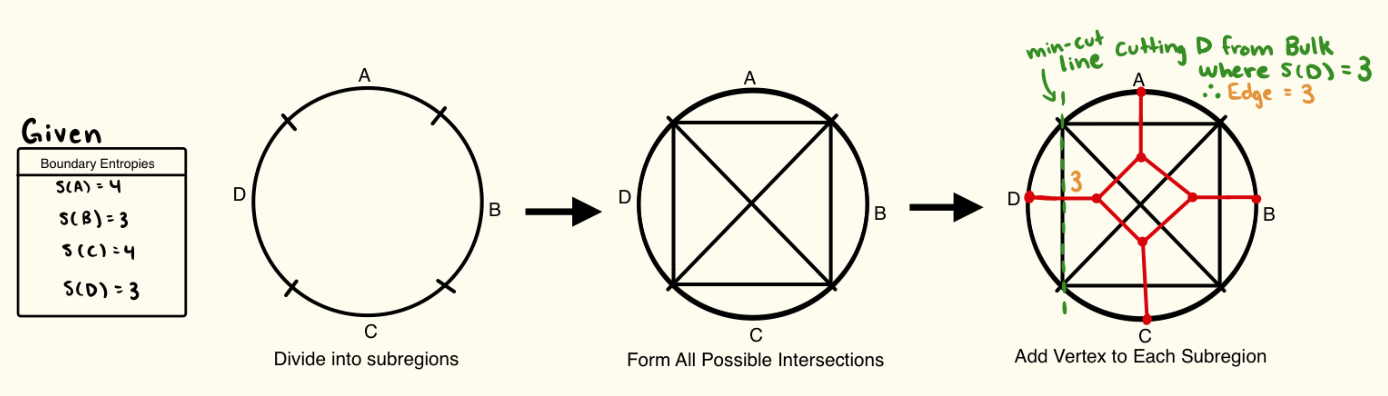
\includegraphics[width=\textwidth]{vertex_subregions.jpeg}  % Adjust width as needed
    \caption{This illustration shows the process of DBRP and demonstrates a simple min-cut for a single subregion (D). The key challenge of the DBRP is finding a set of edge weights such that ALL possible min-cuts match ALL given boundary entropies simultaneously. For more complex combinations like S(ABC), S(ABD), etc., additional entropy constraints must be implemented to ensure the solution accurately represents the entanglement structure of the boundary theory.}  % Caption text
    \label{fig:single subregion min-cut}  % Label for referencing
\end{figure}

\subsection{Entropy Constraints}
To ensure a solution exists where all possible min-cuts match all given boundary entropies. We \textbf{need} the following properties:
In order to illustrate following properties I will introduce a complete set of entropy values for a 4-region system. Let A, B, C, D be the four atomic regions.

\begin{figure}[htbp]
    \centering
    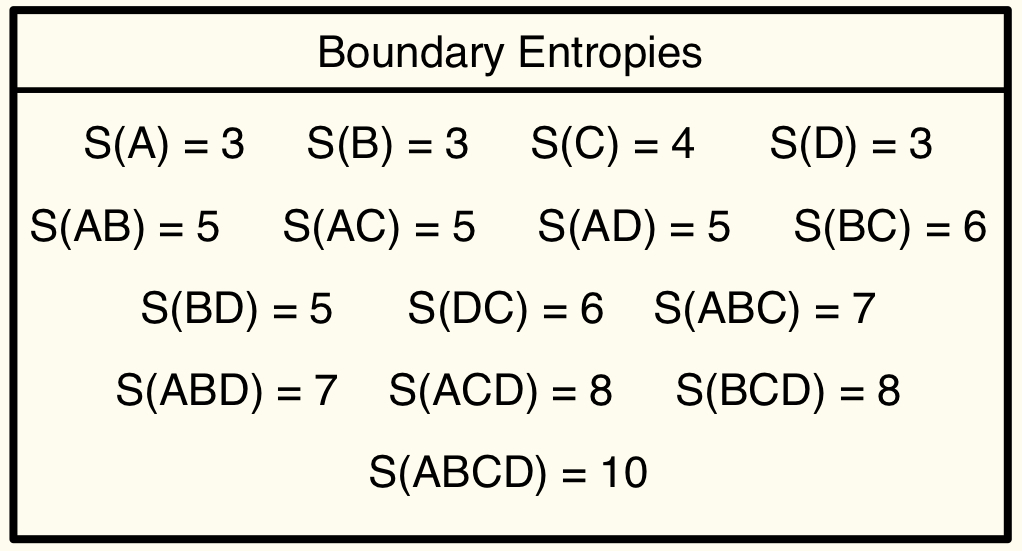
\includegraphics[width=.7\textwidth, height=.22\textheight]{values.jpeg}  % Adjust width as needed
    \caption{Full Entropies of 4 region system}
\end{figure}

\newpage

\begin{enumerate}
    \item \textbf{Subadditivity (SA)}: Entropy of combined system is at most the sum of information in the individual components.
    This property ensures redundancy exists when storing information across multiple locations. This means potential information overlaps between components, which ensures recovery mechanisms.
    \begin{figure}[htbp]  % 'h' places the figure "here" (can be adjusted)
        \centering
        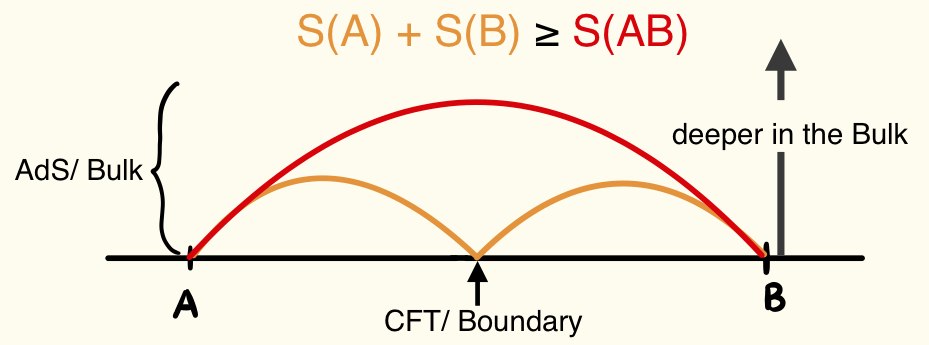
\includegraphics[width=0.8\textwidth,height=0.2\textheight]{sa.jpeg}  % Adjust width as needed
        \caption{The red line value has to be less than or equal to the sum of orange line values in order to ensure subadditivity.}  % Caption text
        \label{fig:Subadditivity}  % Label for referencing
    \end{figure}
    \\
    We can illustrate this property on our example from above (Fig. 3).
    \begin{figure}[htbp]  % 'h' places the figure "here" (can be adjusted)
        \centering
        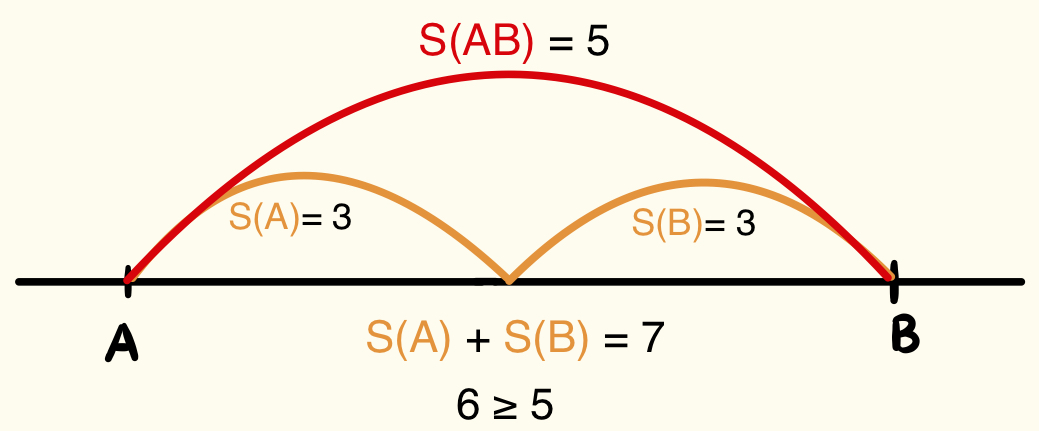
\includegraphics[width=0.75\textwidth,height=0.2\textheight]{sa_ex.jpeg}  % Adjust width as needed
        \caption{In this example property 1 holds. Therefore, edge weight for AB is valid!}  % Caption text
        \label{fig:Subadditivity Example}  % Label for referencing
    \end{figure}

    \newpage

    \item \textbf{Strong Subadditivity (SSA)}: This property extends the concepts of SA to three or more subregions. This property ensures that information overlap exists across three or more components.
    \begin{figure}[htbp]  % 'h' places the figure "here" (can be adjusted)
        \centering
        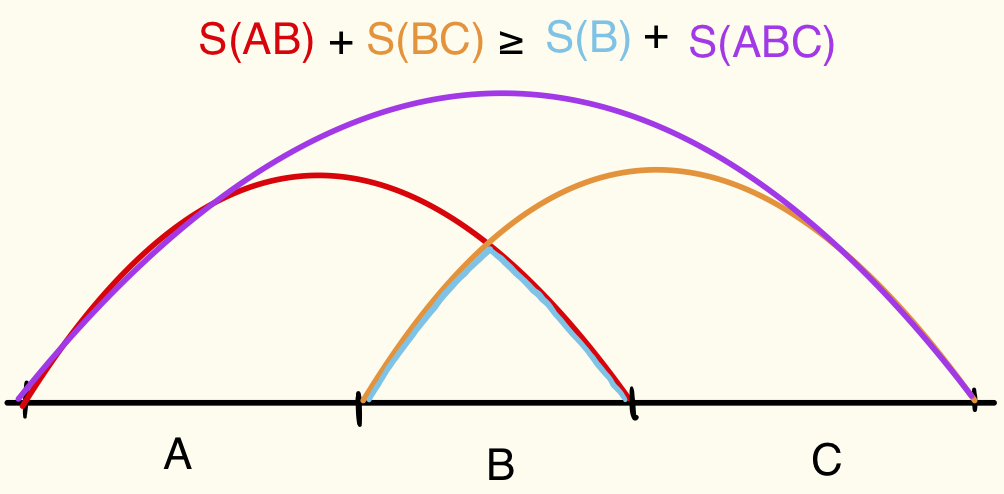
\includegraphics[width=0.75\textwidth,height=0.23\textheight]{SSA.jpeg}  % Adjust width as needed
        \caption{This illustration demonstrates Strong Subadditivity (SSA) on boundary/bulk entropy relationships. In order for the entropy of the ABC subregion to be valid, the sum of entropies S(ABC) + S(B) must be less than or equal to the sum of entropies S(AB) + S(BC).}  % Caption text
        \label{fig:SSA}  % Label for referencing
    \end{figure}
\end{enumerate}
We can illustrate this property on our example from above (Fig. 3). Where S(BC) = 5.
\begin{figure}[htbp]  % 'h' places the figure "here" (can be adjusted)
    \centering
    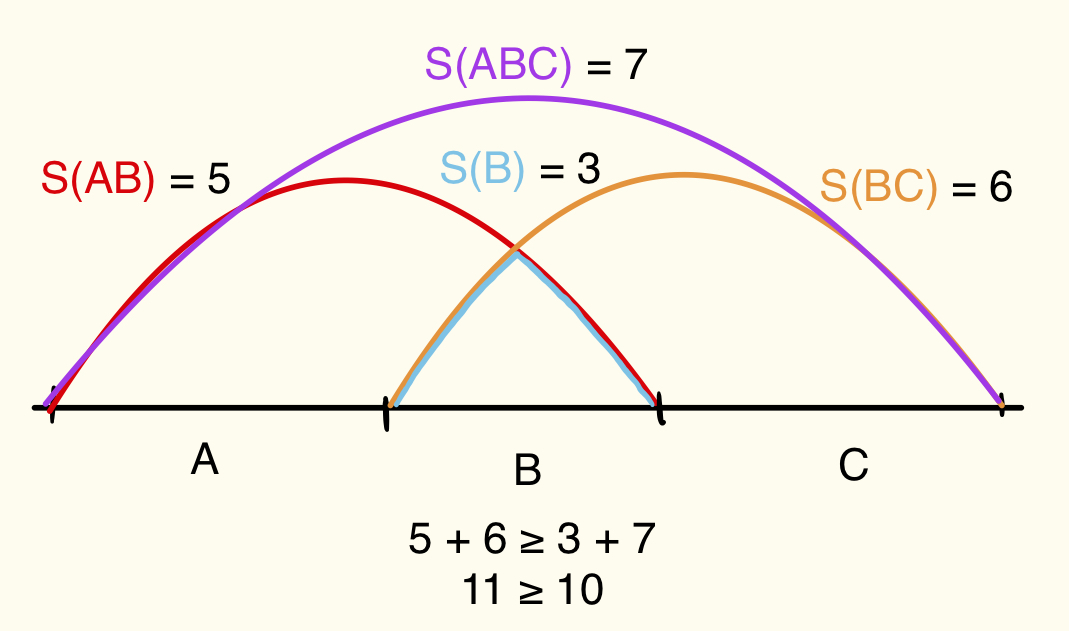
\includegraphics[width=0.7\textwidth,height=0.25\textheight]{ssa_ex.jpeg}  % Adjust width as needed
    \caption{In this example property 2 holds. Therefore, edge weight for ABC is valid!}  % Caption text
    \label{fig:SSA_ex}  % Label for referencing
\end{figure}


\newpage

\subsection{Holographic Quantum State}
\hspace{0.5cm} All boundary states in CFT are holographic. Because of this, there is a corresponding interpretation in bulk AdS space. This allows us to perform computations on a lower-dimensional bounday with no gravity, which then gives us information about higher-dimensional gravity in bulk space, like I stated above (1.3 Holographic Principle). 
\\
But in order for a holographic quantum state to be valid it \textbf{must} satisfy the following property:
\vspace{0.3cm}
\\\textbf{Monogamy of Mutual Information (MMI)}: 
\[
S(AB) + S(BC) + S(AC) \geq S(A) + S(B) + S(ABC)
\] 
\begin{figure}[htbp]  % 'h' places the figure "here" (can be adjusted)
    \centering
    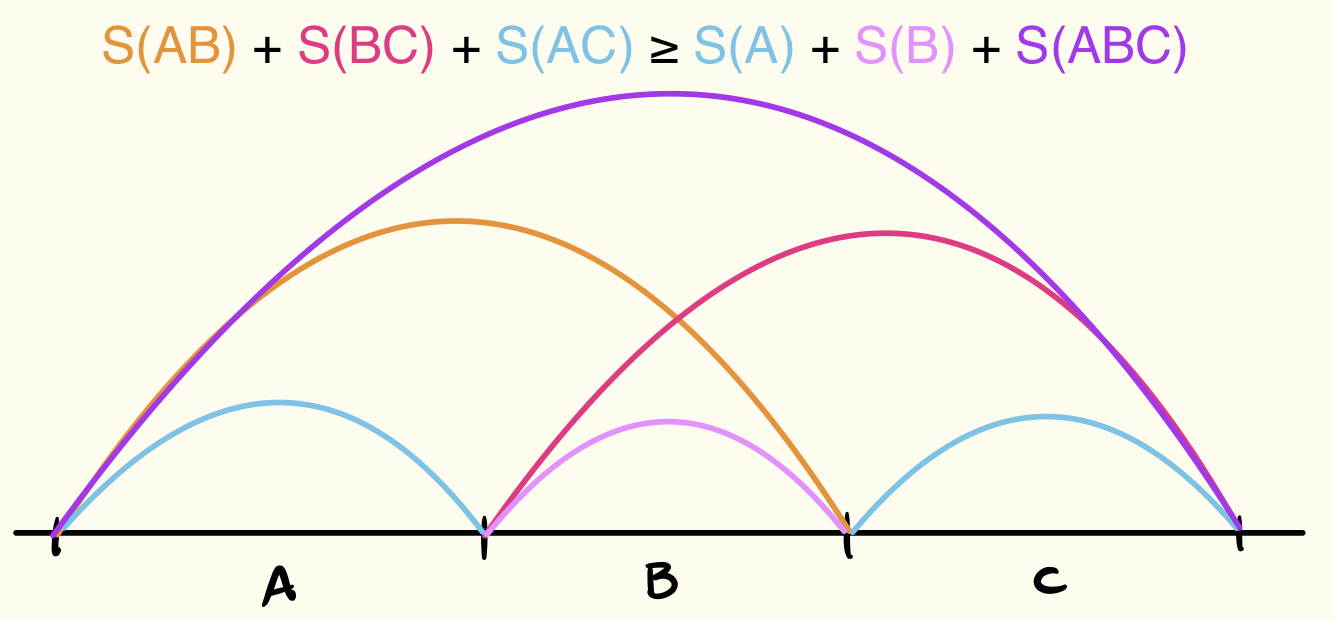
\includegraphics[width=0.9\textwidth, height=0.25\textheight ]{mmi.jpeg}  % Adjust width as needed
    \caption{This illustration represents the property of MMI in the boundary/ bulk. Where S(AC) is equal to the entropy value of A $\cup$ C.}  % Caption text
    \label{fig:mmi}  % Label for referencing
\end{figure}


This property represents an additional constraint beyond SSA for holographic entanglement entropy. It ensures the fact that mutual information shared between three regions cannot be arbitrarily distributed. In order for us to utilize DBRP the entanglement entropy must be holographic. This ensures graph produced corresponds to given geometric space. 
\\
\\
We can represent this property on our example from above (Fig. 3). 
\[
6 + 7 + 7 \geq 4 + 4 + 9
\]
\[
20 \geq 17
\]

\subsection{Extended DBRP?}
\hspace{0.5cm} Is it possible to generalize the DBRP to an unknown set of regions? Instead of given a complete set of entanglement structure of the boundary is it possible to create a min-cut graph without a full entanglement structure? I.e. if we have some unknown regions can we find real-valued entropy of said unknown regions?

\section{DBRP on 4D Hilbert Space}
\hspace{0.5cm} DBRP is typically performed in higher-dimensional settings but for simplification purposes we will explore DBRP the simpliest form possible. In order to use DBRP there needs to be entanglement entropy, which requires at least two subsystems. Therefore, we will look at a system with two qubits.
\\

A 4D Hilbert space represents two qubits, therefore the total space is: 
\[
    \mathbb{C}^2 \otimes \mathbb{C}^2 = \mathbb{C}^4
\]
(Where $\mathbb{C}^2$ represents a single qubit becuase a single qubit can either represents $|0\rangle$ or $|1\rangle$)
\\
To perform DBRP on a higher-dimensional Hilbert space, take the tensor product of each Hilbert space to create one large Hilbert space.
    \[
    \mathcal{H}_{\text{total}} = \mathcal{H}_1 \otimes \mathcal{H}_2 
    \]

    \begin{figure}[htbp]
        \centering
        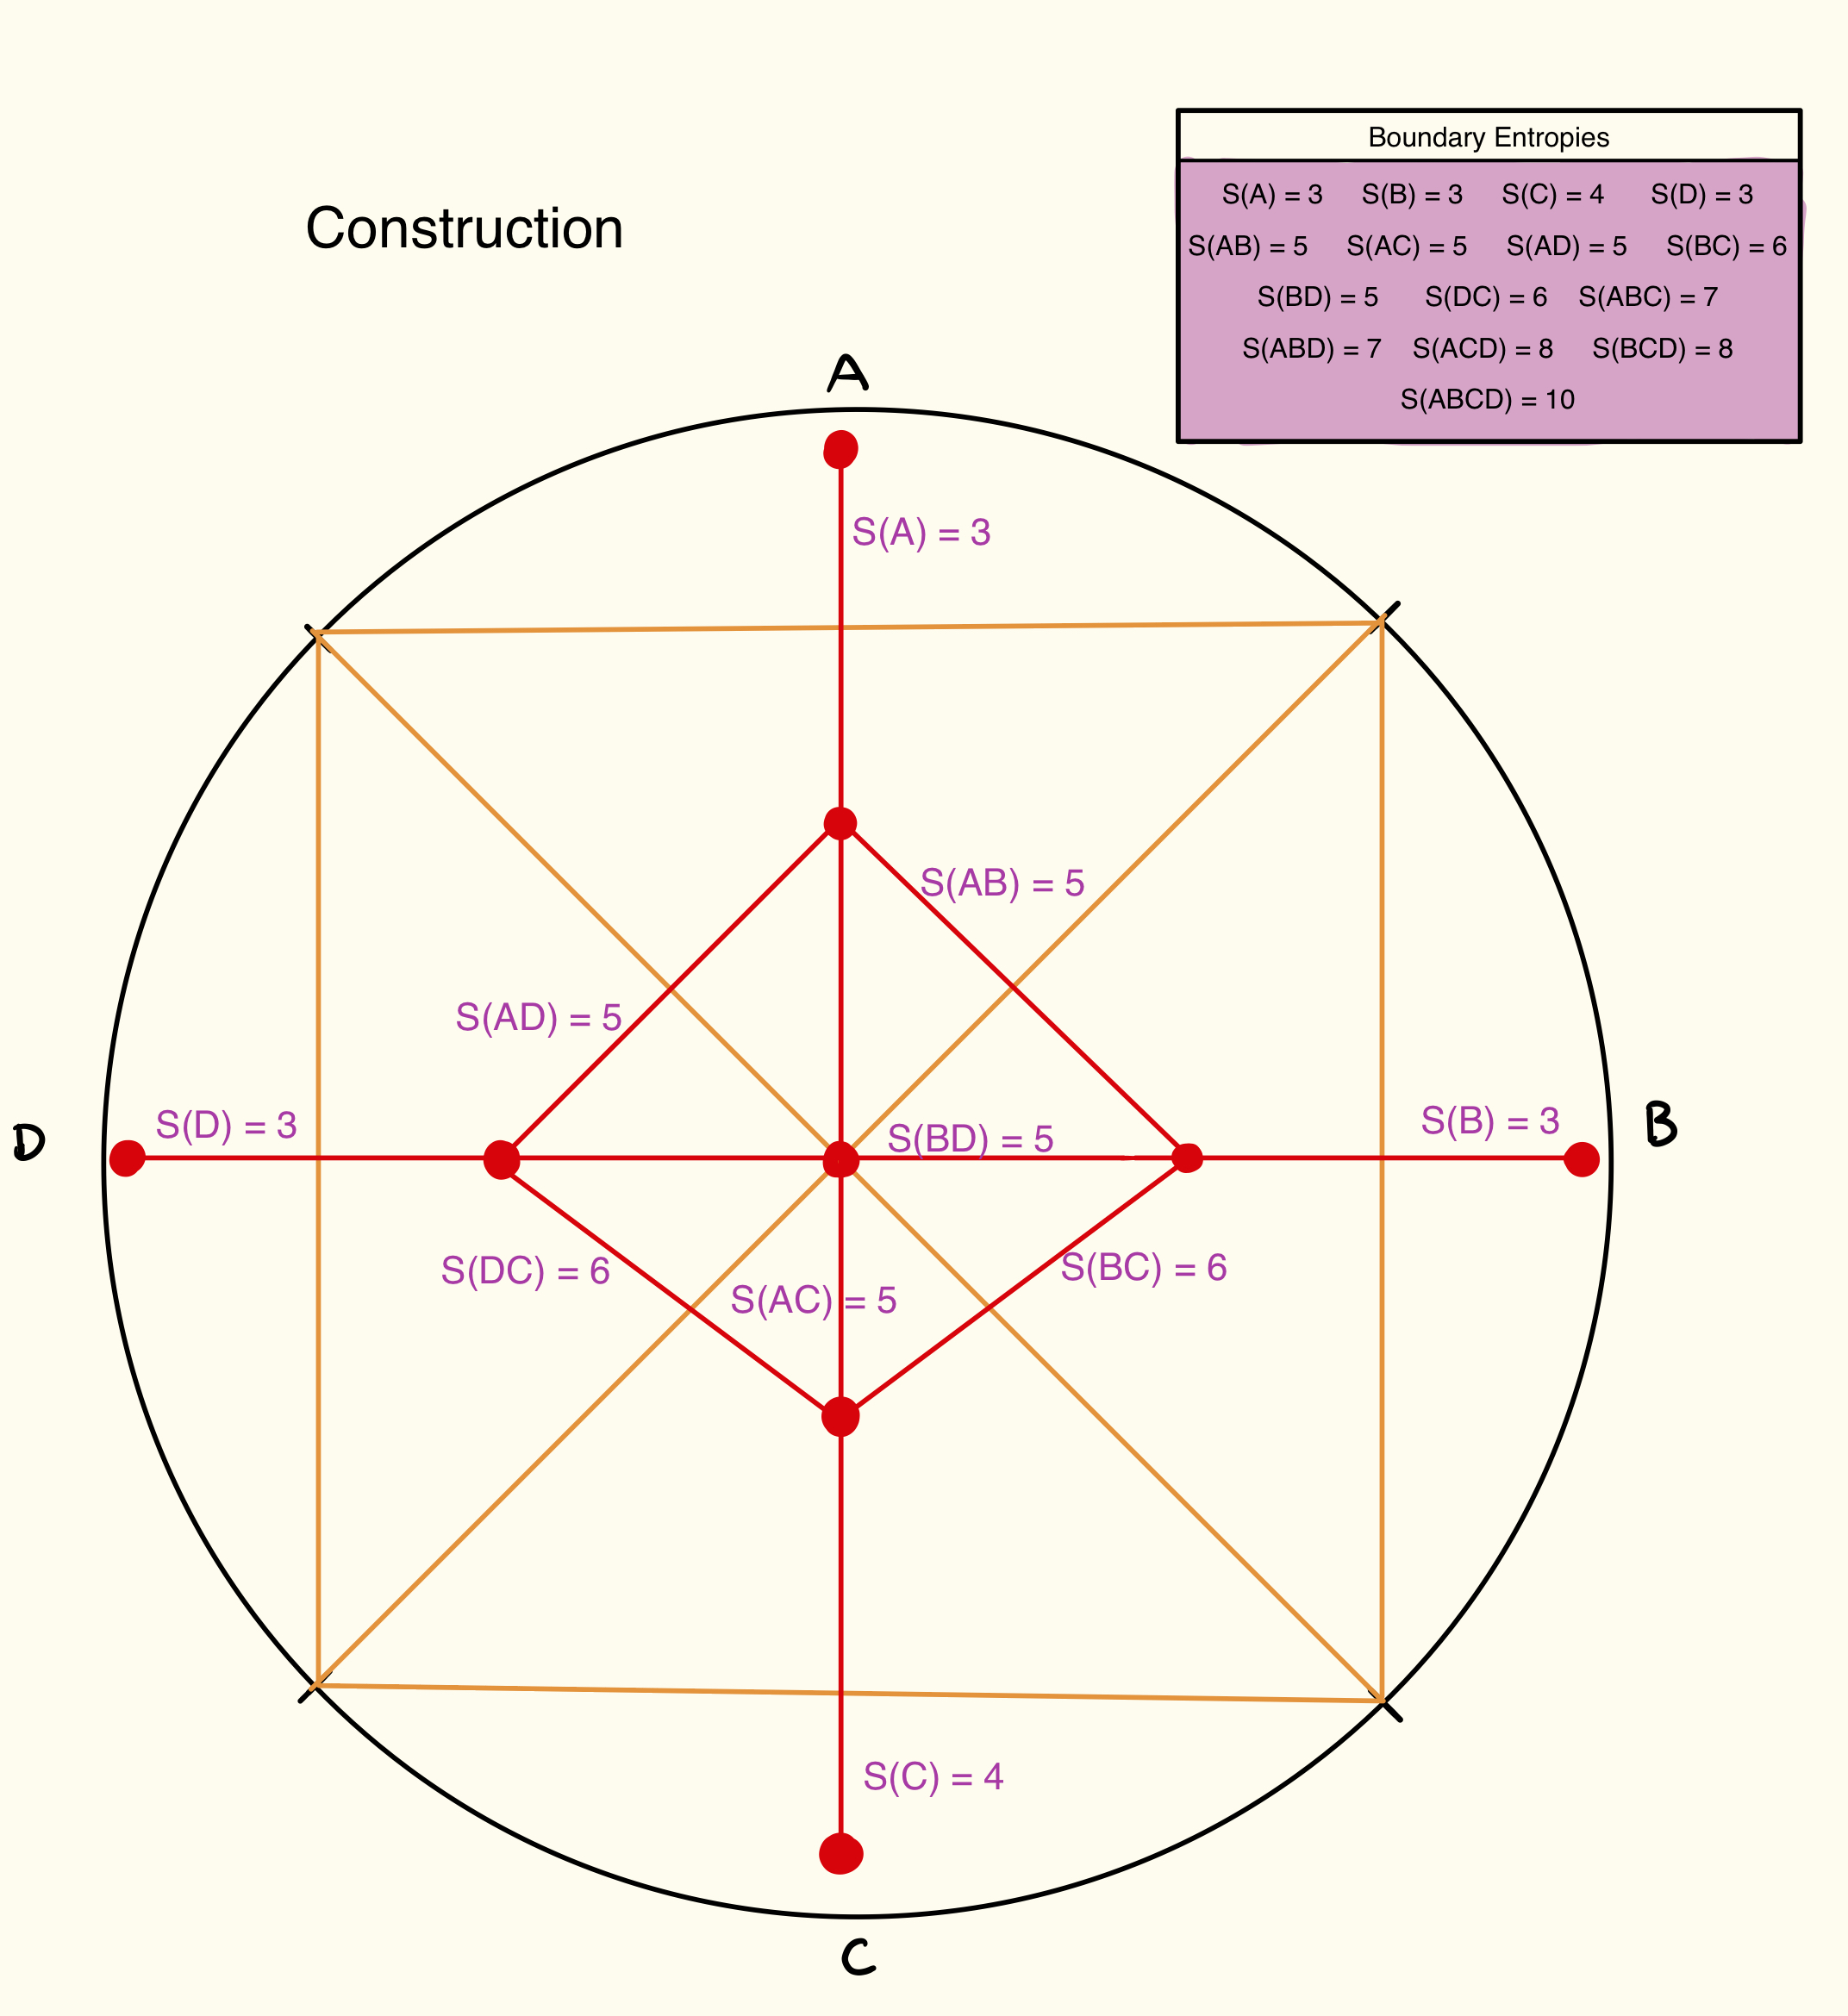
\includegraphics[width=\textwidth]{construction.jpeg}  
        \caption{This illustration shows the process of Fig. 3, adding entanglement entropies to edges.}  
        \label{fig:construction}  
    \end{figure}

\newpage 

We then can use min-cut properties to verify all entanglement entropies and properties hold for constructed graph.

In order to fully construct the bulk graph for the set of entanglement entropies from example above we will have to penetrate "deeper" into the bulk in order to find the minimal edge for the min-cut. In order to simplify the illustration of min-cut I am going to introduce a new set of entanglement entropies so I can demonstrate min-cut between subregions.

Given set of entropies: 
\[
    S(A) = 3, S(B) = 3, S(C) = 4, S(D) = 3, S(AD) = 5
\]
\begin{figure}[htbp]
    \centering
    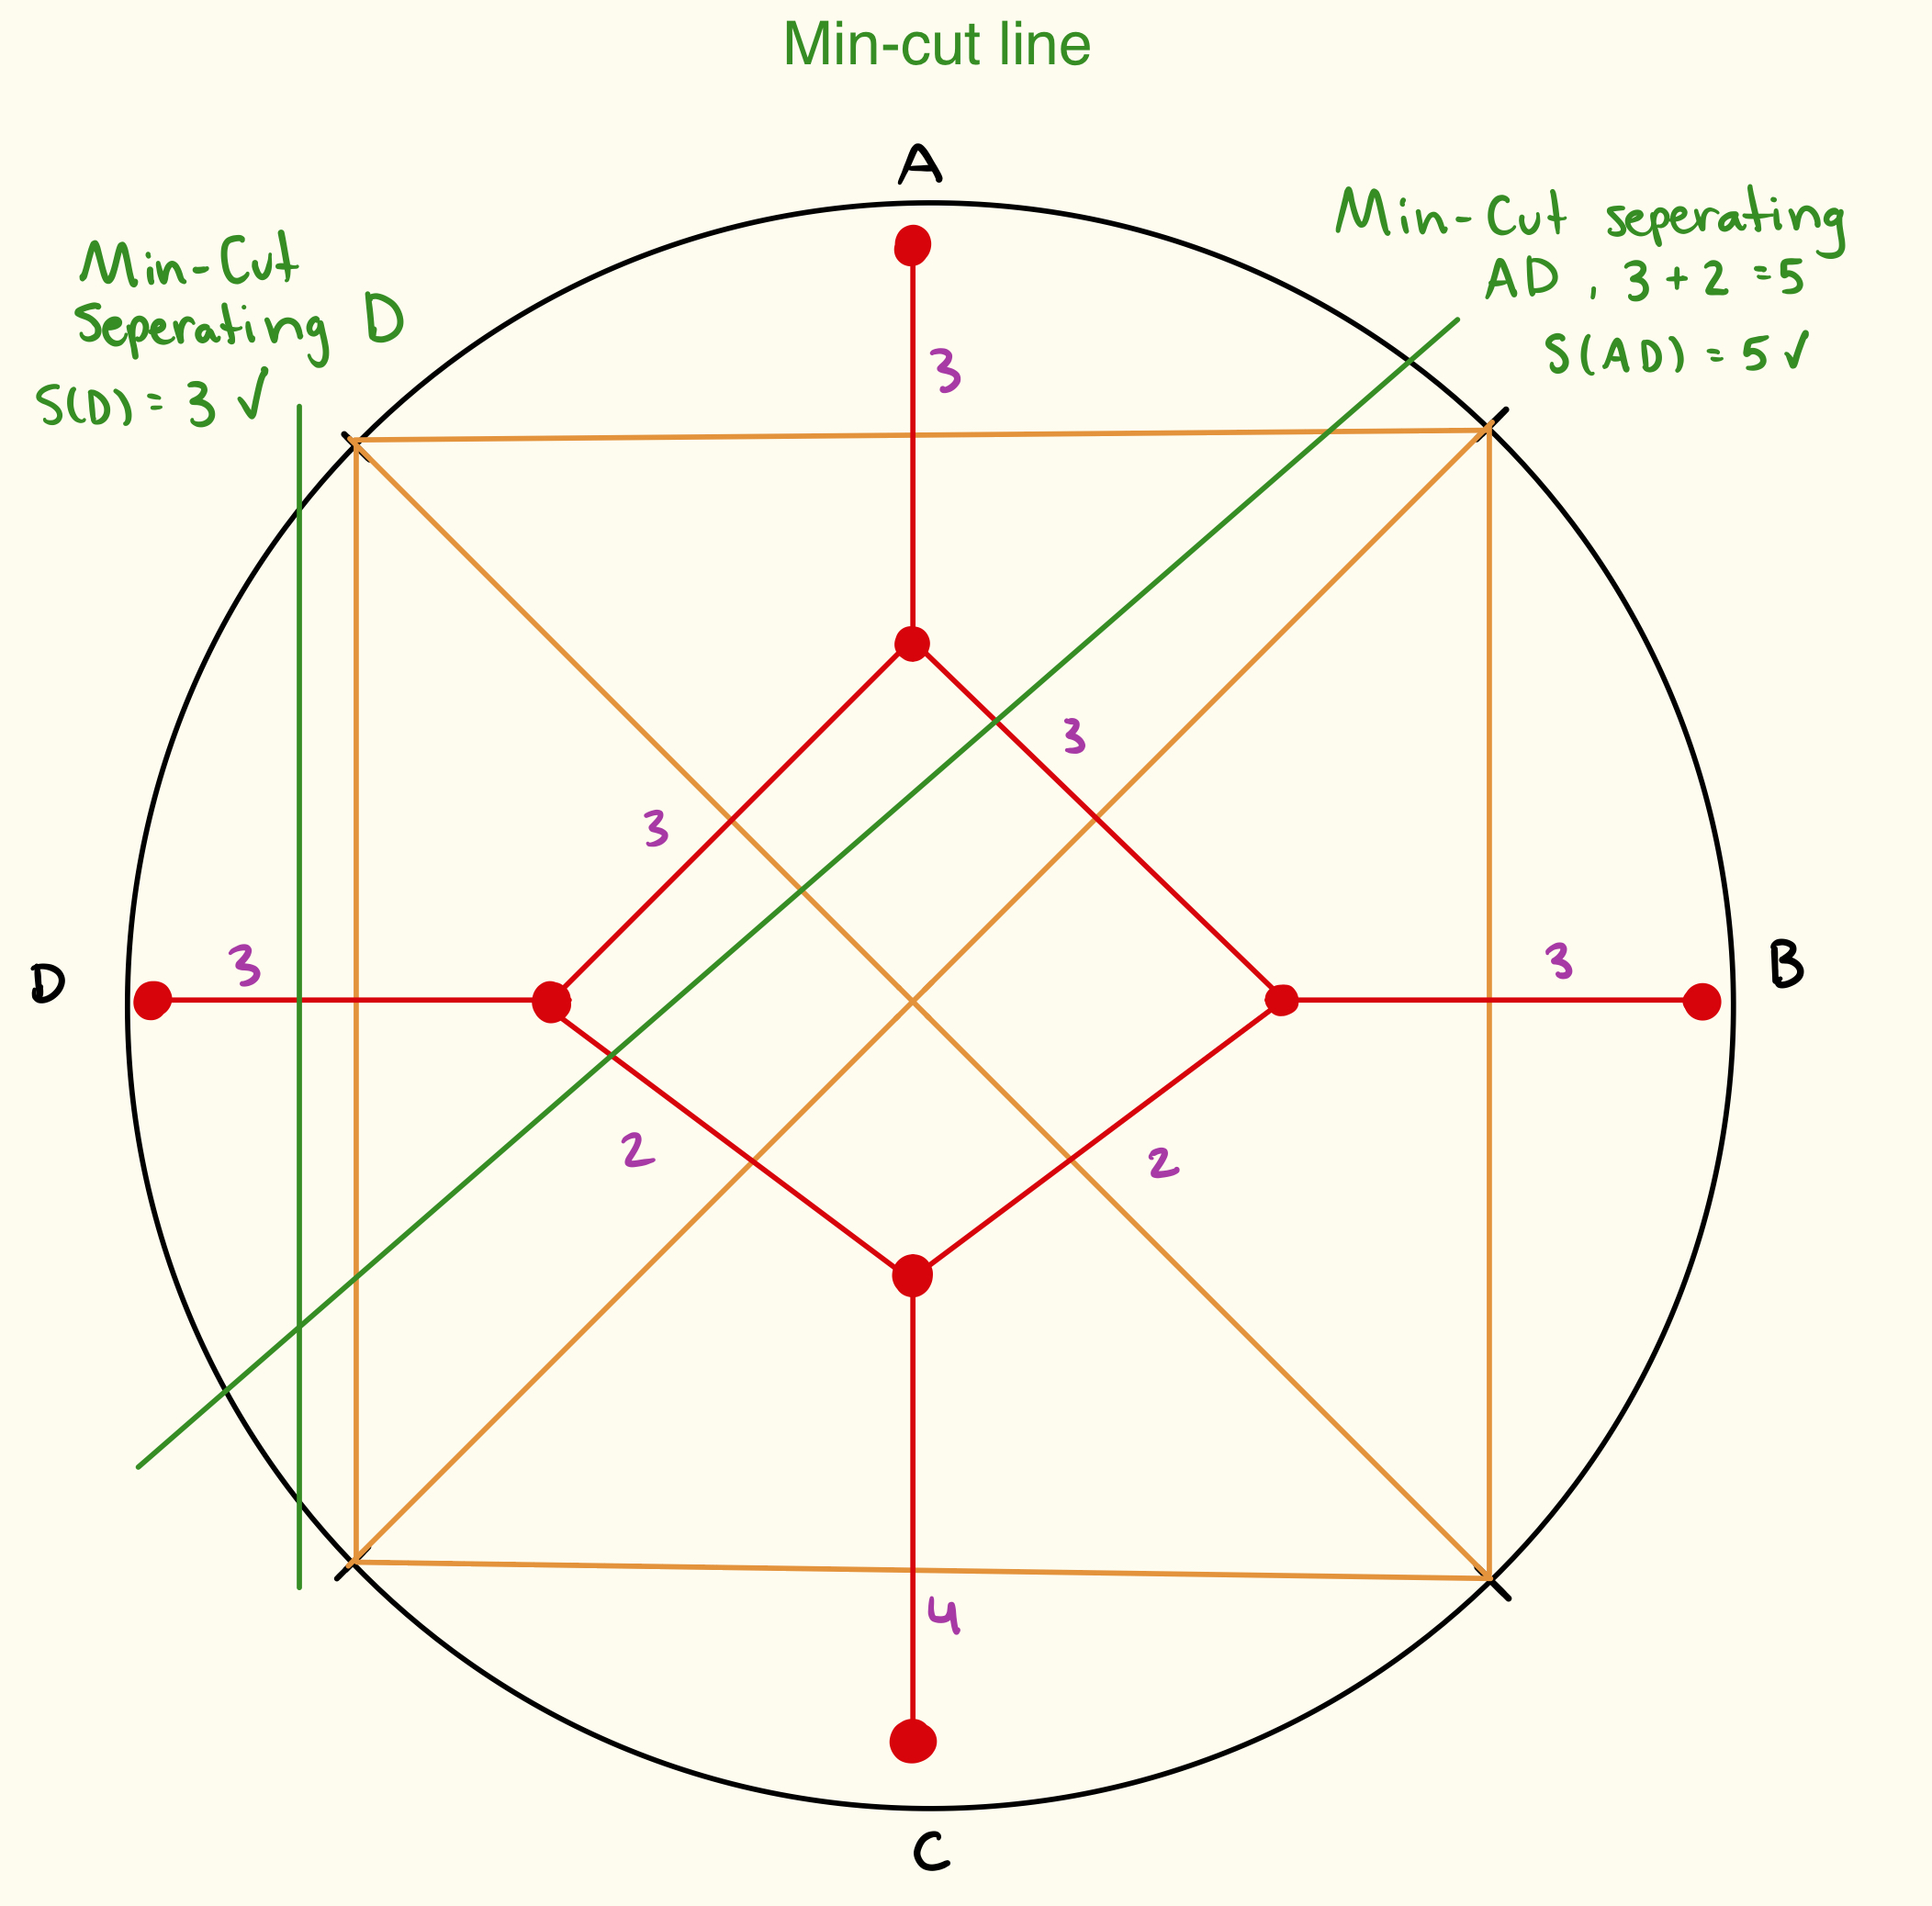
\includegraphics[width=\textwidth]{mincut.jpeg}  
    \caption{This illustration shows how to use min-cut in order to verify edge weights.}  
    \label{fig:mincut example}  
\end{figure}

Edge weight values of A, B, C, D, are implied because there is only one possible edge for these values to be on. But as we penetrate deeper into the bulk these values are unknown. This is when we will introduce linear programming in order to determine the weights of edges as we penetrate deeper into the bulk. We then use min-cut in order to verify edge weights chosen are correct (as shown in illustration).
\\

Penetrating deeper in the bulk can be visulized on the illustration I included above (Fig. 1).

\begin{figure}[htbp]
    \centering
    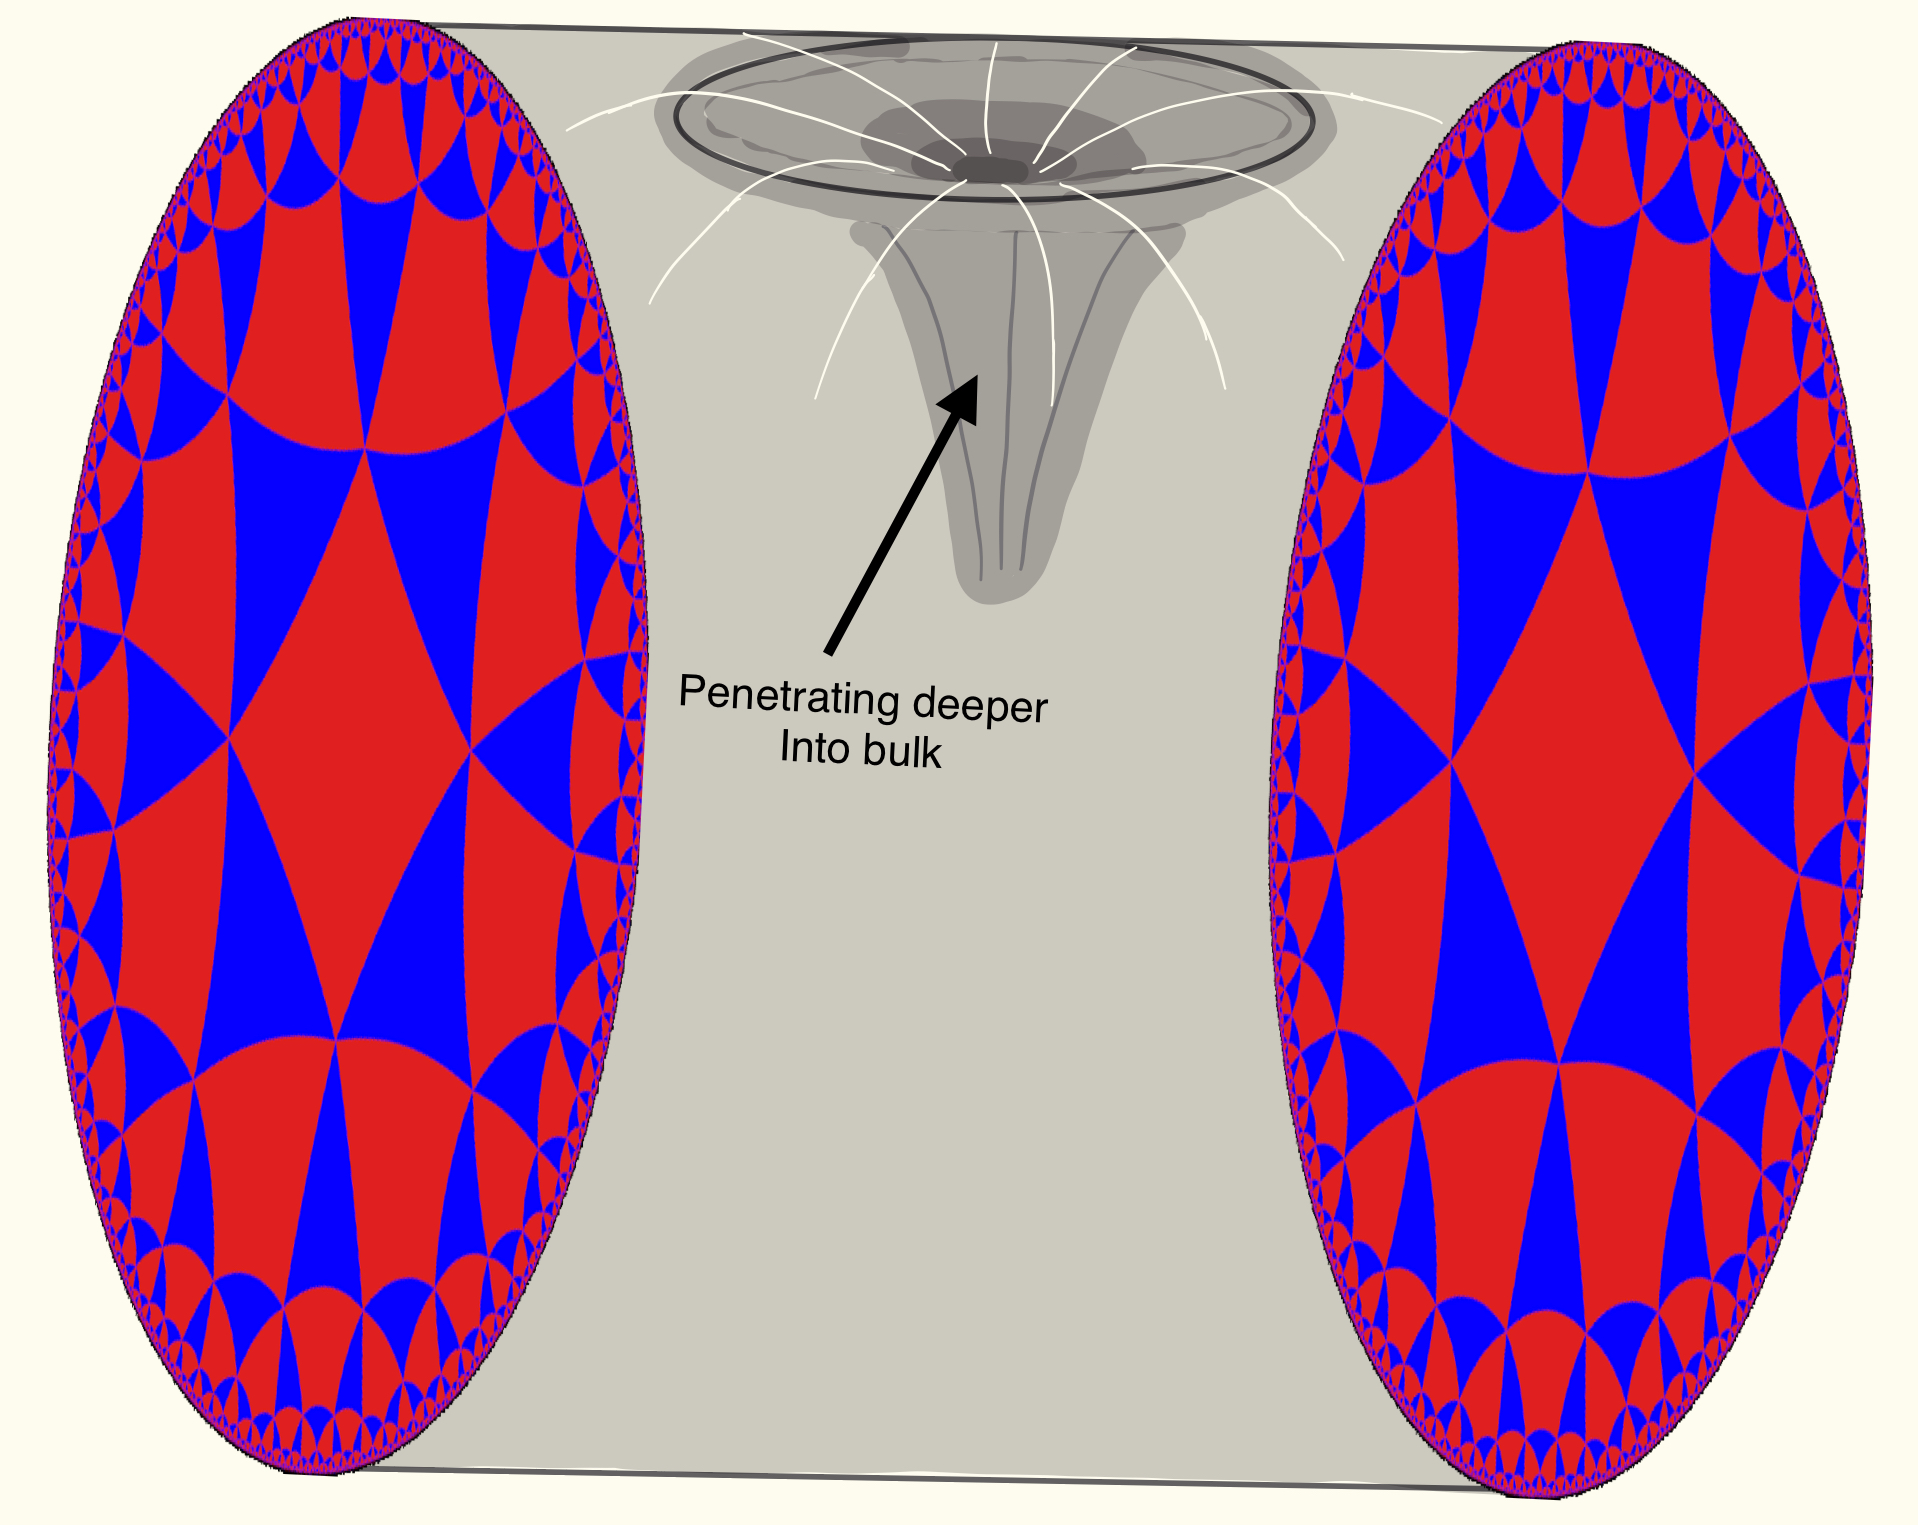
\includegraphics[width=\textwidth]{deeper.jpeg}  
    \caption{This illustration shows what it looks like to penetrate deeper in the bulk to find min-cut edges.}  
    \label{fig:penetrating bulk}  
\end{figure}

\newpage

\begin{center}
    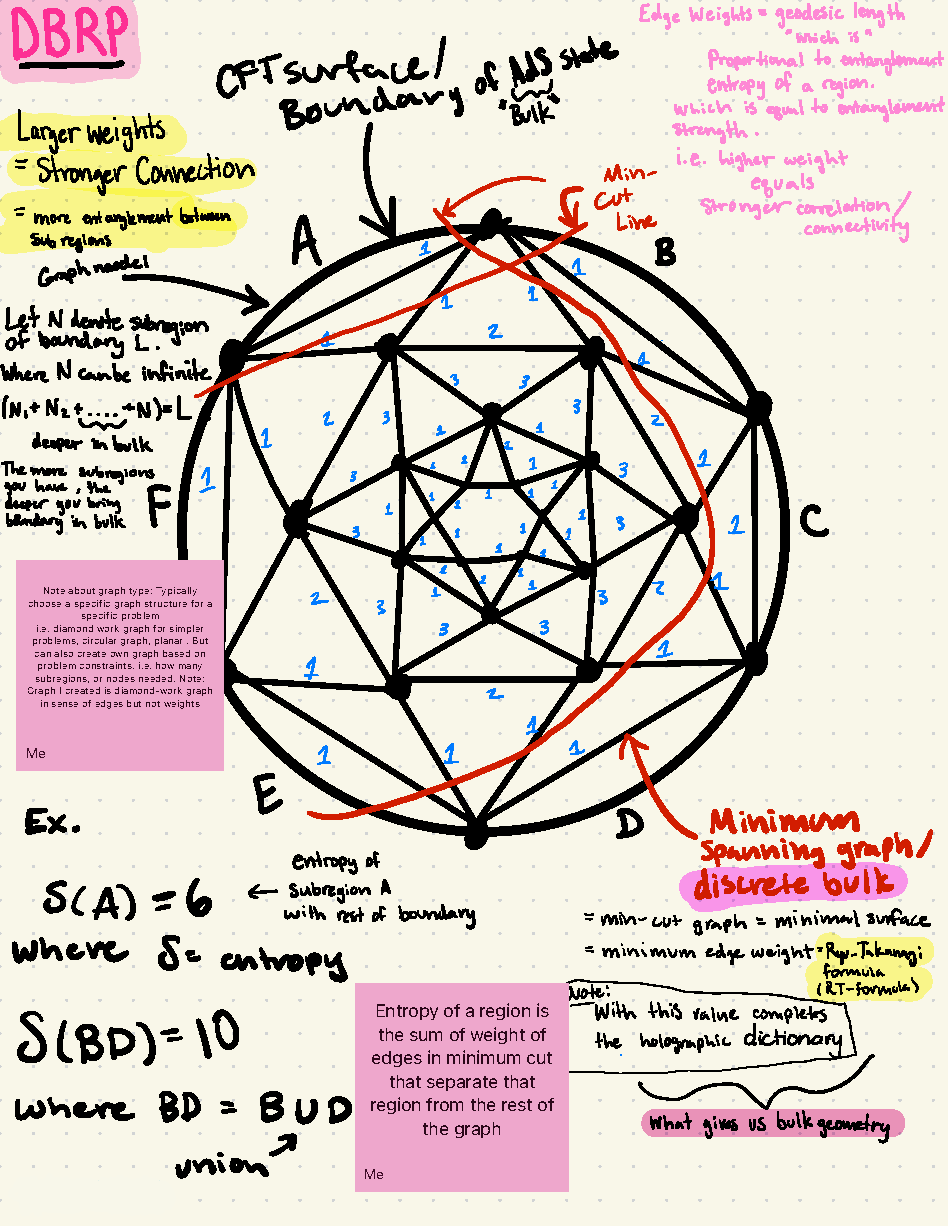
\includegraphics[width=0.8\textwidth]{dbrp_summed.pdf}
\end{center}

\section{Conclusion}
Summarize key findings, limitations, and possible future research directions

\newpage

%%%%%%%%%%%%%%%%%%%%% REFERENCES %%%%%%%%%%%%%%%%%%%%%%%
\begin{thebibliography}{9}
    \bibitem{example}
    Scott Aaronson and Jason Pollack, \textit{Discrete bulk reconstruction}, 2023.
    \bibitem{2}
    Ronak Ramachandran, \textit{Further Exploration of the Discrete Bulk Reconstruction Problem}, 2023.
    \bibitem{AI}
    ChatGPT
\end{thebibliography}

\end{document}

